\chapter{Deep Learning for Genotype-by-Environment Prediction of Maize Grain Yield}\label{ch3:gxe}

\section{Introduction}
Genotype-by-environment (G$\times$E) interactions are a key mechanism underlying crop stability and performance \cite{lopez2023leveraging,rogers2021importance}. Accurately modeling these interactions has important practical implications, including increased food security and optimized farming practices \cite{ray2013yield}. Because the G$\times$E contribution to grain yield variation is substantial, yield rankings are not stable across environments; a hybrid superior in one site or year may be inferior in another \cite{rogers2021importance,lopez2023leveraging}. A breeder who selects on cross-environment mean performance will systematically mis-rank hybrids for the environment of interest. Therefore, predicting within-environment hybrid ordering is critical for improved selection. 

An increase in publicly available data has brought both renewed focus and challenge to G$\times$E prediction. The Genomes to Fields (G2F) Initiative curated a public dataset of genotypes and environments, which spans multiple years, hybrids, and field sites \cite{lopez2023leveraging}. Each yield observation carries both the genotype and the environmental covariates of the plot it was grown in, so a model can represent G$\times$E interactions directly. The 2024 G2F prediction competition built a benchmark on this dataset and standardized the task with a common dataset \comment{repeats the word "dataset"}, a held-out target year, and a single evaluation metric \cite{g2f-2024-competition}. This design makes independently developed methods directly comparable. The competition scores predictions by the Pearson correlation within each environment \comment{well, technically only the 2025 comp (manuscript in prep) did}, averaged across environments, which gives relative ranks priority over absolute scale \cite{g2f-2024-competition}. Additionally, since this dataset was collected in real-world field conditions, it contains heterogeneous data sources with varying quality and extensive missingness. By addressing these constraints, models developed on this dataset are more likely to generalize to real-world breeding scenarios.

A variety of methods have been developed for G$\times$E prediction. Early genomic prediction approaches relied on statistical models such as genomic best linear unbiased prediction (GBLUP) \cite{vanraden2008efficient} and Bayesian linear mixed models \cite{meuwissen2001prediction} to predict breeding values purely from genotypes. These methods were later extended to add genotype-by-environment covariance structure, either through explicit modeling of environmental covariates \cite{crossa2017genomic,heslot2014integrating} or kernel-based approaches \cite{jarquin2014reaction}. Although these methods have proven effective for G$\times$E prediction in some scenarios, they are limited by several inductive biases. The interaction structure must be specified a priori in the case of kernel methods, which prevents flexible modeling of complex relationships. Furthermore, these methods assume a linear relationship between inputs and outputs, which limits the depth of interactions that can be learned. In the case of G$\times$E prediction, this is particularly limiting because the relationship between genotype and environment is often nonlinear \cite{montesinos2021review}.

By contrast, deep learning models are a natural extension for multimodal genomic prediction because they can learn nonlinear feature hierarchies from heterogeneous inputs \cite{azodi2019benchmarking,montesinos2024multimodal}. Prior studies have applied multilayer perceptrons (MLPs) to compute structured interaction components \cite{montesinos2018multi}, combined genotype and weather data to predict yield directly \cite{shook2021crop}, and used sequence models, including state-space and transformer architectures, to model marker sequences \cite{caduceus,snvformer,wu2023transformer}.

However, when a wide range of modeling strategies were evaluated head-to-head in the first public G2F prediction competition, which used the 2022 season as its held-out target, statistical and deep learning models both produced satisfactory yield estimates with no family separating decisively from the rest \cite{g2f-maize-2025}. This result suggests that no single model class guarantees better accuracy on this task. Multimodal architectures for genomic prediction commonly encode each modality with its own encoder and combine the resulting representations late, through concatenation, a weighted sum, or a dedicated fusion layer \cite{montesinos2024multimodal, shook2021crop}. Under this paradigm, marker--environment interactions can only be formed after each modality has been processed independently, so the interactions available to the model are limited to those that survive compression. This design leaves an open question: whether direct interactions between individual marker and environmental tokens improve G$\times$E prediction \comment{if we say "open question", do we need to formulate the next clause as a question? otherwise, I feel like it kinda reads oddly}.

We designed this study to test whether a unified marker and environment representation could outperform branch-based late fusion for G$\times$E prediction. We trained the FullTransformer \comment{this is the first time mentioning "the FullTransformer," need to introduce it properly} with the 2024 G2F competition data and encoded marker and environmental tokens in one transformer sequence \cite{g2f-2024-competition,attention}. A sparse MoE block supported token-level specialization, and an affine head corrected absolute scale while it preserved within-environment rank. We reviewed 427 run records and selected completed comparisons of fusion architecture, objective choice, and affine calibration. The selected model achieved a macro environment PCC of $0.423$ and MSE of $55.40$; this result corresponds to sixth place in the retrospective comparison. Future work will test whether new data and feature representations can close the gap to the competition-winning PCC of $0.45$ \comment{after disqualification, comp winning number is now 0.436, and we would be third place}.

\section{Methods}
\subsection{Data}
Data for this model were obtained through the 2024 Genomes to Fields (G2F) Maize Prediction Competition \cite{g2f-2024-competition}. The dataset included trait, metadata, soil, weather, genotype, and environmental covariate files spanning the 2014-2024 growing seasons, with yield labels for 2014-2023 released prior to the competition, and 2024 labels made publicly available after the competition's end. The training dataset contained 173,960 trait rows across 272 environments; 164,921 of those rows had finite yield. The 2024 test dataset contained 10,057 submission-template rows across 23 environments. Raw genotype data contained 5,899 hybrid records with 2,425 single nucleotide variant (SNV) marker loci. Environmental data contained 654 numeric environmental covariates (ECs), along with 16 daily weather variables and separate metadata and soil tables. 

The data were collected across many sites, years, and management regimes, so they are heterogeneous and carry extensive missingness. The competition organizers deliberately released much of the data in raw form to capture the difficulty of modeling real-world data. Extensive preprocessing, including filtering and imputation, was necessary to address inconsistencies and ensure reliable performance. We detail the steps taken to clean our marker and environmental data in Sections~\ref{sec:ch3-marker-preproc} and~\ref{sec:ch3-env-preproc} respectively.

\subsubsection{Marker Data}\label{sec:ch3-marker-preproc}
The raw numerical genotype table contained 5,899 hybrid records and 2,425 candidate SNV loci. The raw marker files stored these states as $0$, $0.5$, and $1$, so at each locus, we encoded alleles by dosage according to the scheme in Table~\ref{tab:ch3-vocabulary} to make them compatible with tokenization. A value of $2$ represents two major alleles, a value of $1$ represents a heterozygous pair of alleles (major-minor), and a value of $0$ represents two minor alleles. 

\begin{table}[htbp]
    \centering
    \renewcommand{\arraystretch}{1.5}
    \begin{tabular}{@{} l c @{}}
        \toprule
        \textbf{Allele Combination} & \textbf{Model Token} \\
        \midrule
        Major-Major (\textit{AA}) & 2 \\
        Major-Minor (\textit{Aa}) & 1 \\
        Minor-Minor (\textit{aa}) & 0 \\
        \bottomrule 
    \end{tabular} 
    \caption{Genomic Input Marker Encodings. Each diploid marker is encoded as a single token representing the dosage of the major allele by multiplying the raw dosages ($0$, $0.5$, $1$) by two.}
    \label{tab:ch3-vocabulary}
\end{table}

Marker data preprocessing consisted of filtering and imputation, which we applied to the released all-hybrid genotype table. We removed loci with more than $10\%$ missing values. This process removed 201 loci, leaving 2,224 locus inputs to our final model. Additionally, phenotype rows without a corresponding genotype were dropped, decreasing the training set from 164,921 to 163,026 rows.

For the reported model, missing marker calls were processed sequentially in genotype-file order. For each missing call, we calculated the locus-specific median among genotype records sharing either parent with the target hybrid. Missing loci were replaced with the corresponding median value. Because records were processed sequentially, values imputed for earlier records could contribute to the donor medians used for later records. In total, this procedure filled 104,820 missing calls. After imputation, dosage values were multiplied by two and rounded to the nearest integer to produce model tokens. This conversion affected 2,516 imputed calls whose values fell outside the raw $\{0, 0.5, 1\}$ dosage grid; ordinary heterozygous calls at $0.5$ converted exactly to token $1$.

\subsubsection{Environmental Data}\label{sec:ch3-env-preproc}
In addition to genotypic data, we cleaned environmental data in a multi-step process. First, we focused on the output column, which measured grain yield in megagrams per hectare (Mg/ha) and served as the prediction target. We excluded all rows which lacked either yield measurements or complete environmental data. Of the 173,960 raw trait rows, 9,039 lacked a finite yield value and were dropped. From the 163,026 rows that retained both a finite yield and a matching genotype record (Section~\ref{sec:ch3-marker-preproc}), we further removed rows without seasonal weather data, yielding 161,803 records, and rows without EC coverage, yielding 143,050 records. These plot records corresponded to 238 unique environments. Because 34 environments lacked complete weather or EC blocks, they were excluded from the final cohort.

After applying these filters, we performed imputation on the weather station location data included in the competition dataset. For weather stations with partially missing data, we replaced missing observations with the station's mean latitude/longitude coordinates over all existing years. One research station, location TXH4, had no location data present. We used the Texas Tech New Deal Research farm \cite{txh4} as a proxy to retrieve the coordinates for this station, since both are located in Lubbock, Texas. We used the facility's official website to retrieve the New Deal Research Farm's latitude and longitude.

In addition to imputing weather-station locations, we compressed the daily weather data into 46 summary features. First, we indexed the 16 daily weather variables by environment and date, and dropped five variables \comment{which 5 variables? why?}, reducing the daily weather set to 11. We then aggregated variables starting on the planting date, and ending 14 days after harvest for historical environments and on the last date supplied in the seasonal-weather record for 2024 environments. For each retained weather variable, we calculated the minimum, maximum, mean, and accumulated sum over the aggregation window, yielding 44 summary features. We added the starting month and number of included days as additional features.

Following filtering and imputation, we integrated our location, weather, and environmental covariate datasets into a unified set of 705 variables, which consisted of 654 ECs, 46 weather summaries, two coordinates, and three categorical fields. In the best run, the three categorical fields (\texttt{Irrigated}, \texttt{Treatment}, and \texttt{Previous\_Crop}) were excluded, leaving 702 numeric environmental covariates as model inputs. Continuous variables were standardized to zero mean and unit variance, and the scaler was fit only on the training set to prevent data leakage.

We applied the same coverage requirements to the 2024 benchmark rows. Of the 10,057 submission-template rows across 23 environments, 9,486 rows across 22 environments entered the benchmark cohort. The filters removed all 385 rows of environment \texttt{SCH1\_2024}, so that environment does not appear in the cohort or in any reported benchmark result. The remaining 186 excluded rows came from 13 environments that were retained.

\subsection{Model Architecture}\label{sec:ch3-architecture}
\subsubsection{Overview}
We developed the FullTransformer, a full-sequence transformer model that predicts maize yield as a function of genotype and environment. The model represents marker dosages and environmental covariates in one token sequence, allowing self-attention to model genotypic, environmental, and G$\times$E structure in a shared representation space. A sparse mixture-of-experts (MoE) feed-forward sublayer \cite{shazeer2017outrageously} adds capacity through token-level expert routing, and a learned \texttt{[CLS]} summary token \cite{bert} provides the representation used for rank prediction. An environment-conditioned affine-calibration branch converts the rank prediction into the final yield estimate. The architecture is summarized in Figure~\ref{fig:ch3-fullarch}.

\begin{figure}[t]
    \centering
    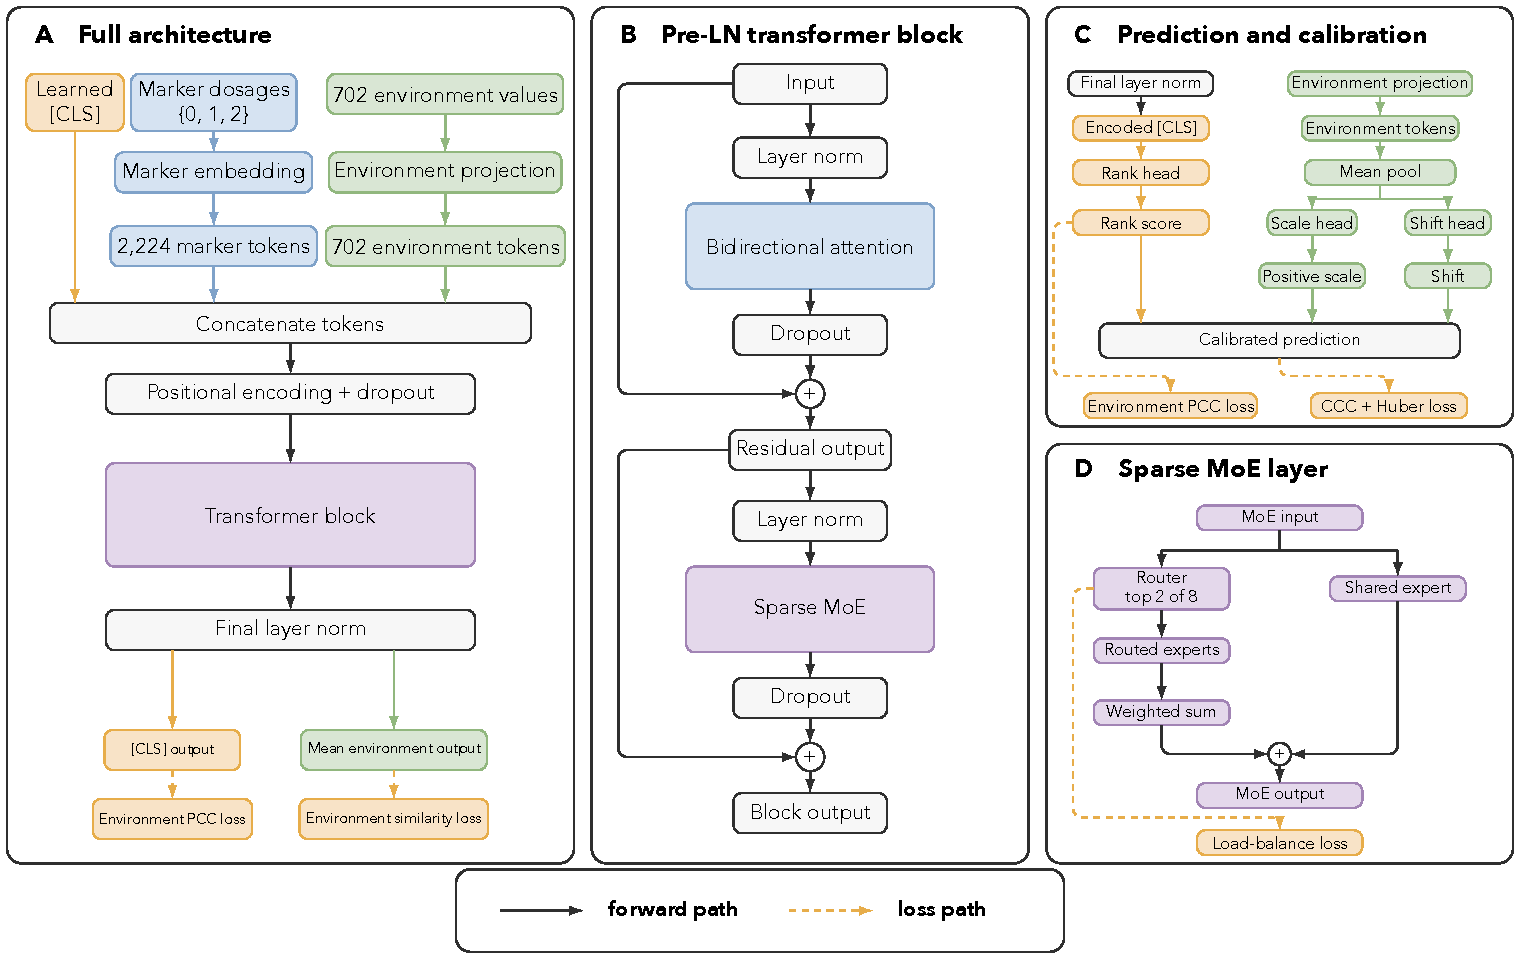
\includegraphics[width=\linewidth]{figures/gxe-tf/fulltransformer-architecture.pdf}
    \caption{ \comment{this fig shows up after all the prose. Any way to move it up? Let's also remove the box around the legend.} FullTransformer architecture for maize yield prediction. (A) The model embeds 2,224 marker dosages and projects 702 environmental values into one sequence with a learned \texttt{[CLS]} token. One transformer block produces the normalized \texttt{[CLS]} and environmental representations used by the primary and auxiliary losses. (B) The pre-layer-normalized block applies bidirectional attention and a sparse MoE layer with dropout and residual connections. (C) \comment{i think that A) and C) are slightly misaligned here in terms of how they convey the environmental input} The rank head predicts relative yield, while the mean projected environmental representation supplies a positive scale and shift for affine calibration. The environment PCC loss acts on the rank score, and the CCC and Huber losses act on the calibrated prediction. (D) \comment{maybe have dotted lines from the MoE block in B) indicating the "expanded" view of the MoE} The MoE router selects two of eight routed experts per token and combines their weighted output with one shared expert. A load-balance loss discourages routing collapse. Blue blocks show marker and attention operations, green blocks show environment operations, purple blocks show MoE operations, and orange blocks show \texttt{[CLS]} and losses. Solid arrows show forward paths, and dashed arrows show loss paths.}
    \label{fig:ch3-fullarch}
\end{figure}

\subsubsection{Input Representation}
For the reported model, each sample was represented by a sequence of length $2{,}927$: one learned \texttt{[CLS]} summary token, 2,224 marker tokens, and 702 environmental tokens. Marker dosages in $\{0,1,2\}$ were embedded with a shared learned lookup table of vocabulary size three and width 256. The same learned \texttt{Linear(1,256)} projection was applied to every standardized environmental scalar, producing one token per environmental feature. The \texttt{[CLS]}, marker, and environmental tokens were concatenated in that order, and a static sinusoidal positional encoding \cite{attention} was added to the sequence. This produced a per-sample encoder input of shape $2{,}927 \times 256$.

Because yield prediction depends on the complete input rather than autoregressive next-token prediction, no causal attention mask was applied. Bidirectional attention \cite{bert} allowed every marker and environmental token to attend to every other position, enabling direct marker--environment interactions within the shared representation.

\subsubsection{Transformer Encoder with Mixture-of-Experts}
The reported FullTransformer used one encoder block with hidden width $256$ and four bidirectional attention heads. The block followed the pre-layer-normalized residual organization used in GPT-2 \cite{gpt2}, with layer normalization applied before each sublayer \cite{layernorm}. The normalized token representations were passed through multi-head self-attention, and dropout with rate $0.15$ was applied to the attention output before it was added to the block input through a residual connection \cite{he2016deep}. The updated token representations were normalized again and passed through the MoE sublayer, whose output received the same dropout before the second residual addition.

The reported encoder replaced the conventional dense feed-forward sublayer with a sparse MoE layer \cite{shazeer2017outrageously}. A learned linear router produced eight logits, one for each routed expert, for every sequence token, including \texttt{[CLS]}, marker, and environmental tokens. The two routed experts with the highest logits were selected independently for each token, and a softmax over those logits produced weights used to combine their outputs. Each routed expert was a two-layer FFN with hidden width $256$, GELU activation, and output width $256$. An additional shared expert with the same structure processed every token, and its output was added to the weighted sum of routed-expert outputs. During training, an auxiliary load-balancing loss with weight $0.01$ discouraged routing collapse by encouraging routing mass to remain distributed across the eight routed experts. This design increased conditional capacity while activating only two routed experts, in addition to the shared expert, for each token. \comment{should we add that this block is visualized in figure 1?}

\subsubsection{Prediction and Calibration Heads}
After the final transformer block, layer normalization was applied to the full sequence. The normalized representation at the \texttt{[CLS]} position was passed through a \texttt{Linear(256,1)} head to produce a scalar rank prediction. This rank head was optimized directly against the environment PCC loss described in Section~\ref{sec:ch3-training}.

The selected model additionally applied an environment-conditioned affine calibration to transform the rank prediction into an absolute-yield prediction. For each sample, we took the mean of its 702 projected environmental input tokens, computed before positional encoding and transformer processing. Every plot record within one environment carried the same environmental covariates, so this mean was constant within an environment; we therefore write it as $\bar{\mathbf z}_E$ for environment $E$. Two learned \texttt{Linear(256,1)} heads, $f_s$ and $f_b$, mapped $\bar{\mathbf z}_E$ to a scalar raw-scale value and a scalar shift, respectively. The calibrated total prediction was computed as

\begin{equation}\label{eq:ch3-affine-calibration}
    \begin{aligned}
        s_E^{\mathrm{raw}} &= f_s(\bar{\mathbf z}_E), &
        b_E &= f_b(\bar{\mathbf z}_E), &
        f_s,f_b &: \mathbb{R}^{256} \rightarrow \mathbb{R}, \\
        \hat{y}_{\mathrm{total}}
        &= \left[\operatorname{softplus}\!\left(s_E^{\mathrm{raw}}\right)+10^{-4}\right]
        \hat y_{\mathrm{rank}} + b_E.
    \end{aligned}
\end{equation}

The weights of both calibration heads and the bias of the shift head were initialized to zero. The scale-head bias was initialized to the inverse softplus of one, so the initial scale was approximately $1.0001$ after adding the $10^{-4}$ offset, while the initial shift was zero. The softplus activation and offset constrained the scale to be strictly positive. Every hybrid in the same environment shared the same positive scale and shift, so calibration preserved both the within-environment rank ordering and Pearson correlation, leaving the macro environment PCC unchanged while allowing adjustment of absolute yield scale.

The model also exposed the mean of the encoded environmental tokens after the transformer and final normalization for use in the auxiliary environment-similarity loss (Section~\ref{sec:ch3-losses}). This pooled representation was not itself a prediction head; it shaped the learned environmental representation as described below.

\subsection{Training}\label{sec:ch3-training}
\subsubsection{Training Objective}\label{sec:ch3-losses}
The training objective was built around an environment PCC loss designed to mirror the competition's macro environment PCC metric. Within each local per-GPU microbatch, we computed the Pearson correlation between observed yield and the model's rank prediction for every environment $e \in \mathcal{E}_B$ containing at least four observations. Here, $\hat{y}_i$ denotes the rank prediction for sample $i$. Each GPU computed correlations from its local microbatch of 256 samples, and the sufficient statistics were not pooled across GPUs. The raw environment correlations were uniformly averaged without Fisher $z$ transformation or sample-count weighting. The environment PCC loss was defined as

\begin{equation}\label{eq:ch3-pcc}
    r_e =
    \frac{\sum_{i \in e} (y_i - \bar{y}_e)(\hat{y}_i - \bar{\hat{y}}_e)}
    {\sqrt{\sum_{i \in e}(y_i - \bar{y}_e)^2}
     \sqrt{\sum_{i \in e}(\hat{y}_i - \bar{\hat{y}}_e)^2}}.
\end{equation}

\begin{equation}\label{eq:ch3-envpcc}
    L_{\mathrm{envpcc}} = 1 - \frac{1}{|\mathcal{E}_B|} \sum_{e \in \mathcal{E}_B} r_e.
\end{equation}

In addition to optimizing within-environment ranking, we implemented an auxiliary environment-similarity objective to align internal environmental representations with the raw environmental data. We mean-pooled the encoded environmental tokens into an embedding $\mathbf{z}_i$ for each sample $i$. The cosine similarity between $\mathbf{z}_i$ and $\mathbf{z}_j$ defined the learned similarity $S^{z}_{ij}$, while the cosine similarity between their standardized raw environmental vectors defined the target similarity $S^{E}_{ij}$. We computed the loss as the mean-squared difference between these similarities over all off-diagonal pairs in a local microbatch of size $B$:

\begin{equation}\label{eq:ch3-env-sim}
    L_{\mathrm{env\text{-}sim}} = \frac{1}{B(B-1)} \sum_{\substack{1 \leq i,j \leq B \\ i \neq j}} (S^{z}_{ij} - S^{E}_{ij})^2 .
\end{equation}

The maximum weight of this loss was $0.1$. The term was inactive until epoch 50 and then ramped linearly to its maximum weight by epoch 100.

For absolute-yield calibration, the calibrated total prediction was optimized with an environment concordance correlation coefficient (CCC) loss \cite{lin1989concordance} and a mean Huber loss \cite{huber1964robust}. For each environment $e$, the concordance correlation was

\begin{equation}\label{eq:ch3-ccc-loss}
\begin{aligned}
    \rho_{c,e}
    &= \frac{2\,\operatorname{cov}\!\left(y_e,\hat{y}^{\mathrm{total}}_e\right)}
    {\sigma_{y,e}^{2}+\sigma_{\hat{y}^{\mathrm{total}},e}^{2}
    +\left(\mu_{y,e}-\mu_{\hat{y}^{\mathrm{total}},e}\right)^2}, \\
    L_{\mathrm{envCCC}}
    &= 1-\frac{1}{|\mathcal{E}^{(2)}_B|}
    \sum_{e \in \mathcal{E}^{(2)}_B}\rho_{c,e},
\end{aligned}
\end{equation}

where $\mathcal{E}^{(2)}_B$ contained environments in the local microbatch with at least two observations and nonzero yield and prediction variance. The environment CCC loss had maximum weight $0.05$. The Huber loss used mean reduction, $\delta=1.0$, and maximum weight $0.02$. Both calibration terms were inactive until epoch 150 and ramped linearly to their full weights by epoch 250. Until epoch 250, the rank prediction was detached from calibration gradients \comment{what does this mean?}, allowing the calibration heads to learn without altering the rank head. Beginning at epoch 250, calibration gradients reached the rank prediction at $10\%$ of their ordinary magnitude \comment{this is just a weight of 0.1, think that would be clearer to say}, while the environment PCC loss on the rank prediction remained fully active throughout training.

Combining all of these objectives, the total loss function was defined as

\begin{equation}\label{eq:ch3-total-loss}
    L(t) = L_{\mathrm{envpcc}}
    + 0.1\,r_E(t)L_{\mathrm{env\text{-}sim}}
    + r_C(t)\left[0.05L_{\mathrm{envCCC}} + 0.02L_{\mathrm{Huber}}\right]
    + 0.01L_{\mathrm{MoE}},
\end{equation}

where $r_E(t)$ increased linearly from zero to one between epochs 50 and 100, and $r_C(t)$ increased linearly from zero to one between epochs 150 and 250. The final term was the MoE load-balancing loss described above.

\subsubsection{Training Details}
The reported model contained $1{,}552{,}259$ trainable parameters. We trained it on Oak Ridge National Laboratory's Frontier supercomputer using distributed data parallel training across four compute nodes, with eight GPU devices per node. Training used automatic mixed precision with the \texttt{bfloat16} data type. Each GPU processed a microbatch of 256 samples, yielding a global batch size of $4 \times 8 \times 256 = 8192$. The reported run reached early stopping after 53 minutes and 47 seconds of wall-clock time, which corresponds to approximately 29 GPU-hours.

We used the AdamW optimizer \cite{adamW} with weight decay $1 \times 10^{-5}$. The learning rate increased linearly to $1 \times 10^{-4}$ during an approximately five-epoch warmup and then followed cosine decay to a floor of $1 \times 10^{-5}$ over a 400-epoch horizon, defined as $\min(2 \times 200, 3000)$. Training was configured for at most 3000 epochs and stopped early after 200 epochs without improvement in the validation criterion. The model used dropout $0.15$, four attention heads, embedding dimension $256$, one transformer block, and base model and split seeds of 1.

Because the primary objective computed within-environment correlations, we used environment-stratified minibatches with at least 32 samples per represented environment when possible. As described above, correlations were computed within each 256-sample per-GPU microbatch rather than across the global batch. For leave-environment-out validation, we randomly held out $15\%$ of entire pre-2024 environments from model fitting. Checkpoints and early stopping were determined by the macro environment PCC of the rank prediction on this validation subset, with validation loss used to break ties. The 2024 data were excluded from model fitting and checkpoint selection and were subsequently used as a retrospective competition benchmark rather than as an untouched external validation set.

\subsection{Evaluation}
We used the 2024 evaluation data from the G2F competition \cite{g2f-2024-competition} as our retrospective competition benchmark. The competition metric was the macro environment PCC between predicted and observed yield across the 2024 benchmark environments. We retained only rows with finite observed and predicted yields. An environment was eligible for PCC evaluation if it contained at least two observations and both its observed and predicted values were nonconstant. We computed the Pearson correlation within each eligible environment and averaged these correlations uniformly without weighting by environment size. Calibrated total predictions were used to compute the primary reported PCC; rank-head PCC was also calculated for comparison and was equal up to numerical precision because the calibration head applied a constant positive affine transformation within each environment. The evaluation procedure is summarized in Algorithm~\ref{alg:ch3-eval-pcc}.

\begin{algorithm}
\caption{Macro Environment PCC Evaluation}
\label{alg:ch3-eval-pcc}
\begin{algorithmic}
\For{each eligible environment $e \in \mathcal{E}^{\mathrm{valid}}_{2024}$ in the retrospective benchmark}
    \State $y_e \gets$ observed yields for $e$
    \State $\hat{y}^{\mathrm{total}}_e \gets$ calibrated total predictions for $e$
    \State $PCC_e \gets \text{Pearson}(y_e, \hat{y}^{\mathrm{total}}_e)$
\EndFor
\State $PCC_{\mathrm{macro}} \gets \frac{1}{|\mathcal{E}^{\mathrm{valid}}_{2024}|} \sum_{e \in \mathcal{E}^{\mathrm{valid}}_{2024}} PCC_e$
\end{algorithmic}
\end{algorithm}

In addition to the macro environment PCC evaluation, we implemented a macro environment MSE evaluation to assess absolute-yield calibration. We defined the macro environment MSE as 

\begin{equation}\label{eq:ch3-macro-env-mse}
\begin{aligned}
    \mathrm{MSE}_e
    &= \frac{1}{n_e}\sum_{i \in \mathcal{I}_e}
    \left(y_i-\hat{y}^{\mathrm{total}}_i\right)^2, \\
    \mathrm{MSE}_{\mathrm{macro}}
    &= \frac{1}{|\mathcal{E}^{\mathrm{MSE}}_{2024}|}
    \sum_{e \in \mathcal{E}^{\mathrm{MSE}}_{2024}}\mathrm{MSE}_e,
\end{aligned}
\end{equation}

where $\mathcal{I}_e$ is the set of finite observed-prediction pairs in the environment $e$, $n_e$ is the number of such pairs, $\mathcal{E}^{\mathrm{MSE}}_{2024}$ is the set of environments containing at least one finite pair, and $\hat{y}^{\mathrm{total}}_i$ is the calibrated total prediction for sample $i$. In our reported results, $\mathrm{MSE}_{\mathrm{macro}}$ is the macro environment MSE stated alongside the macro environment PCC.

\subsection{Model Development Comparisons}\label{sec:ch3-comparisons}
To evaluate the effectiveness of critical architectural and training choices, we examined run records from the model-development process. We highlight three comparisons: unified versus branch-based processing of markers and environmental covariates, environment PCC versus global MSE training objectives, and uncalibrated versus affine-calibrated predictions. Each comparison was performed on the same 2024 retrospective benchmark and used the same evaluation procedure. Within each comparison, we held the principal settings constant. All six runs used one transformer block, four attention heads, embedding dimension 256, a mixture-of-experts feed-forward layer with eight routed experts, top-2 routing and one shared expert, dropout 0.15, global batch size 8192, microbatch size 256, environment-stratified batching, LEO validation, and the learning rate schedule described in Section~\ref{sec:ch3-training}. The three comparisons were assembled at different stages of development, however, and both the auxiliary losses and the checkpoint-selection criterion changed between those stages. Comparisons therefore hold within a pair and not across pairs.

The first comparison evaluated the performance of a unified transformer block that processed marker and environmental tokens together (Section~\ref{sec:ch3-architecture}) against a branch-based late-fusion model that processed markers and environmental covariates separately before it combined their representations. The branch-based late-fusion model applied a transformer encoder and a parallel LD-oriented CNN to the marker sequence, and an MLP to the environmental covariates. The environment representation was appended to the marker token sequence as a single token, the LD representation was aligned to that sequence and added elementwise, and a layer normalization combined them. A final G$\times$E transformer block processed the fused sequence, and a linear head read the rank prediction from the \texttt{[CLS]} position. Figure~\ref{fig:ch3-branch} shows this architecture. The branch-based late-fusion model contained $2{,}886{,}404$ trainable parameters. These divided into $1{,}452{,}288$ for the marker encoder, $246{,}784$ for the environment encoder, $396{,}288$ for the LD encoder, and $791{,}044$ for the G$\times$E encoder. The unified FullTransformer contained about half as many parameters, so this comparison did not favor the unified model on capacity. At this stage in development, neither model used the environment-similarity auxiliary loss or the affine calibration branch. Both runs in this pair also selected checkpoints on a target-weighted validation score, which reweighted validation locations toward the 2024 site distribution, stabilized each per-location correlation with a Fisher $z$ transformation, weighted it by sample count, and took a pessimistic bootstrap quantile across locations.

\begin{figure}[t]
    \centering
    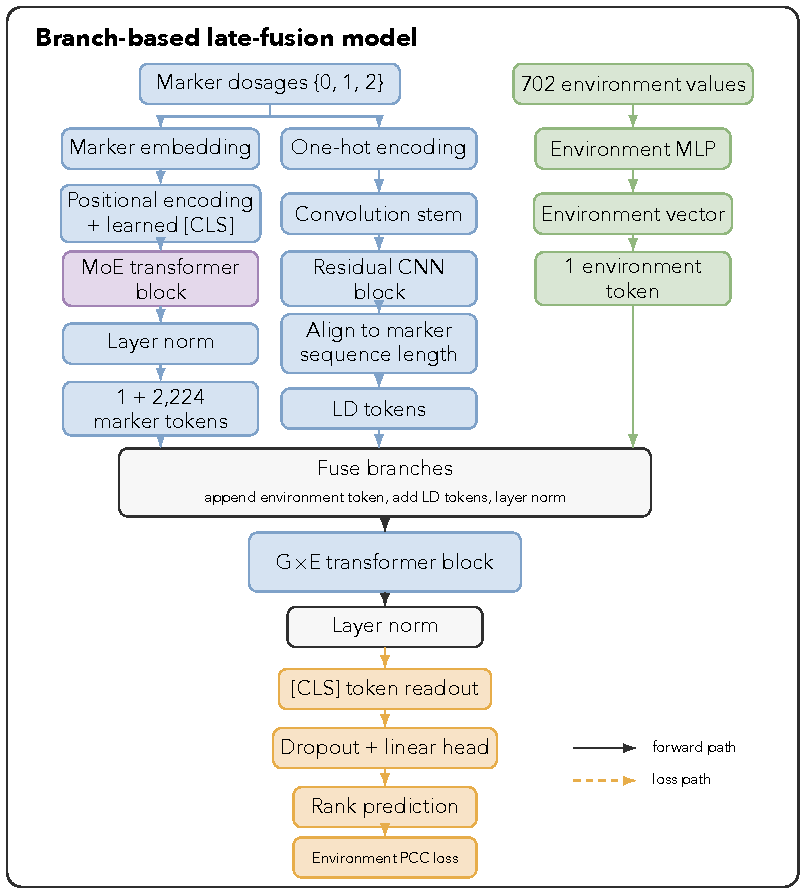
\includegraphics[width=0.78\linewidth]{figures/gxe-tf/branch-architecture.pdf}
    \caption{Branch-based late-fusion model used in the architecture comparison. Marker dosages enter a transformer encoder with a mixture-of-experts feed-forward layer and, in parallel, a one-hot convolutional encoder that captures local linkage-disequilibrium structure. The 702 environmental values enter a multilayer perceptron that produces a single environment token. The environment token is appended to the marker token sequence, the aligned LD representation is added elementwise, and a layer normalization combines them. One G$\times$E transformer block then processes the fused sequence, and a linear head reads the rank prediction from the \texttt{[CLS]} position. Blue blocks show marker operations, green blocks show environment operations, purple blocks show mixture-of-experts operations, and orange blocks show \texttt{[CLS]} and loss operations.}
    \label{fig:ch3-branch}
\end{figure}

The remaining two comparisons came from a later stage of development. Both used the environment-similarity auxiliary loss at weight $0.1$ and selected checkpoints on the macro environment PCC of the rank prediction. After comparing unified and branch-based architectures, we examined the effect of training objective choice. We trained two FullTransformer controls (Section~\ref{sec:ch3-architecture}) with identical architectures and principal hyperparameters, but optimized one model with the environment PCC loss defined in Section~\ref{sec:ch3-losses} and the other with a global MSE loss.

Finally, we compared the effect of the affine calibration head on absolute yield prediction. The reported FullTransformer used the environment PCC loss together with the affine calibration branch, while its control used the environment PCC loss alone. These two runs came from adjacent development commits, so this pair is near-matched rather than exactly matched.

Two runs of the environment PCC configuration completed at the same commit under identical settings. We report both and treat their difference as an estimate of run-to-run variation. Every other comparison arm is a single run, so this study does not yet estimate variation across random initializations. The complete experiment export contained 427 run records, of which 374 finished successfully. The accompanying machine-readable manifest records every exported run, its provenance, completion status, reported metrics, and manuscript disposition. Only completed comparisons from the legacy data scheme entered the primary results; experiments that used the later data-generation or tokenization schemes are designated as future work.

\section{Results}

\subsection{Performance on the 2024 Retrospective Benchmark}
On the 2024 retrospective benchmark, the reported affine-calibrated FullTransformer model achieved a macro environment PCC of $0.423$ and a macro environment MSE of $55.40$. These metrics came from the calibrated total prediction of the checkpoint selected by pre-2024 LEO validation. The result came from one run using seed 1, so no across-seed uncertainty estimate was available.

\subsection{Internal Model Comparisons}
We evaluated architectural and training variants during model development to determine how performance varied across design choices. Section~\ref{sec:ch3-comparisons} defines the three comparisons and the settings that differ between them. In the architecture comparison, the unified FullTransformer control achieved a macro environment PCC of $0.411$ and a macro environment MSE of $96.34$, whereas the branch-based late-fusion model achieved a macro environment PCC of $0.308$ and a macro environment MSE of $116.47$. These results indicate that unified processing of markers and environmental covariates was associated with better within-environment correlation and lower absolute error in this comparison.

Next, we examined how matching the primary training objective to the competition's evaluation metric affected performance. Both models were evaluated with macro environment PCC and macro environment MSE, although one optimized global MSE during training. The model trained with the environment PCC loss achieved a macro environment PCC of $0.423$ and a macro environment MSE of $100.57$. The model trained with the global MSE loss achieved a macro environment PCC of $0.305$ and a macro environment MSE of $14.54$. These results indicate that optimizing within-environment correlation substantially improved macro environment PCC but increased macro environment MSE, suggesting that the resulting predictions were less well-calibrated for absolute yield.

Motivated by this rank--scale trade-off, we compared a near-matched uncalibrated rank model with the reported affine-calibrated model. Both models achieved a macro environment PCC of $0.423$, but their macro environment MSE differed: $101.06$ for the uncalibrated model and $55.40$ for the affine-calibrated model. Calibration improved macro environment MSE by approximately $45.2\%$, while macro environment PCC changed by only $0.00004$. This behavior was expected because an environment-specific affine transformation with a positive scale preserves within-environment Pearson correlation while allowing the absolute scale and offset of the predictions to be adjusted.

The replicate pair described in Section~\ref{sec:ch3-comparisons} bounds how much of this variation is run-to-run noise. Its two runs agreed to three decimals on macro environment PCC at $0.423$, and gave macro environment MSE values of $100.57$ and $101.06$. These differences, $0.0000039$ in PCC and $0.50$ in MSE, provide the study's only estimate of run-to-run variation. On that scale, the $45.66$ MSE improvement from calibration is about 90 times the replicate difference. The corresponding PCC difference of $0.0000378$ amounts to $0.009\%$ of the score. Every other comparison arm is a single run. These results should therefore be interpreted as descriptive model-development comparisons rather than replicated estimates of individual-component effects. Table~\ref{tab:ch3-ablation-summary} reports the highlighted comparisons at full precision.

\begin{table}[htbp]
    \centering
    \footnotesize
    \begin{tabular}{@{}l l c c@{}}
        \toprule
        Comparison & Variant & \makecell{Macro environment \\ PCC} & \makecell{Macro environment \\ MSE} \\
        \midrule
        Architecture & Branch-based late-fusion model & 0.30819 & 116.46976 \\
                     & Unified FullTransformer control & 0.41066 & 96.33830 \\
        \addlinespace
        Training objective & Global MSE & 0.30504 & 14.54242 \\
                           & Environment PCC & 0.42316 & 100.56502 \\
        \addlinespace
        Calibration & Uncalibrated rank model & 0.42317 & 101.06046 \\
                    & Affine-calibrated model & 0.42321 & 55.40464 \\
        \bottomrule
    \end{tabular}
    \caption{Highlighted internal model-development comparisons on the retrospective 2024 benchmark. Comparisons should be made within, rather than across, the three labeled groups. Each row reports a single run. The architecture and objective pairs used matched principal settings; the calibration pair used near-matched runs from adjacent development commits. Values are given to five decimals so that the small differences discussed in the text remain visible. The complete run-level inventory is provided in \texttt{supplement/ablation\_run\_manifest.csv}.}
    \label{tab:ch3-ablation-summary}
\end{table}

\subsection{Performance Across Benchmark Environments}
To better understand the model's performance across environments, we examined variation in PCC among the 2024 benchmark environments (Figure~\ref{fig:ch3-environment-pcc}). All 22 environments in the benchmark cohort met the eligibility criteria described in the Evaluation section and yielded defined PCC values. Across these environments, the model achieved a mean PCC of $0.423$ and a median PCC of $0.434$. The interquartile range of environment-level PCC values was $0.364$--$0.480$, and the full range was $0.247$--$0.567$. The model achieved positive PCC in all 22 environments, with 16 of 22 ($72.7\%$) having PCC greater than $0.40$. Thus, performance was consistently positive but varied meaningfully among benchmark environments.

\begin{figure}[p]
    \centering
    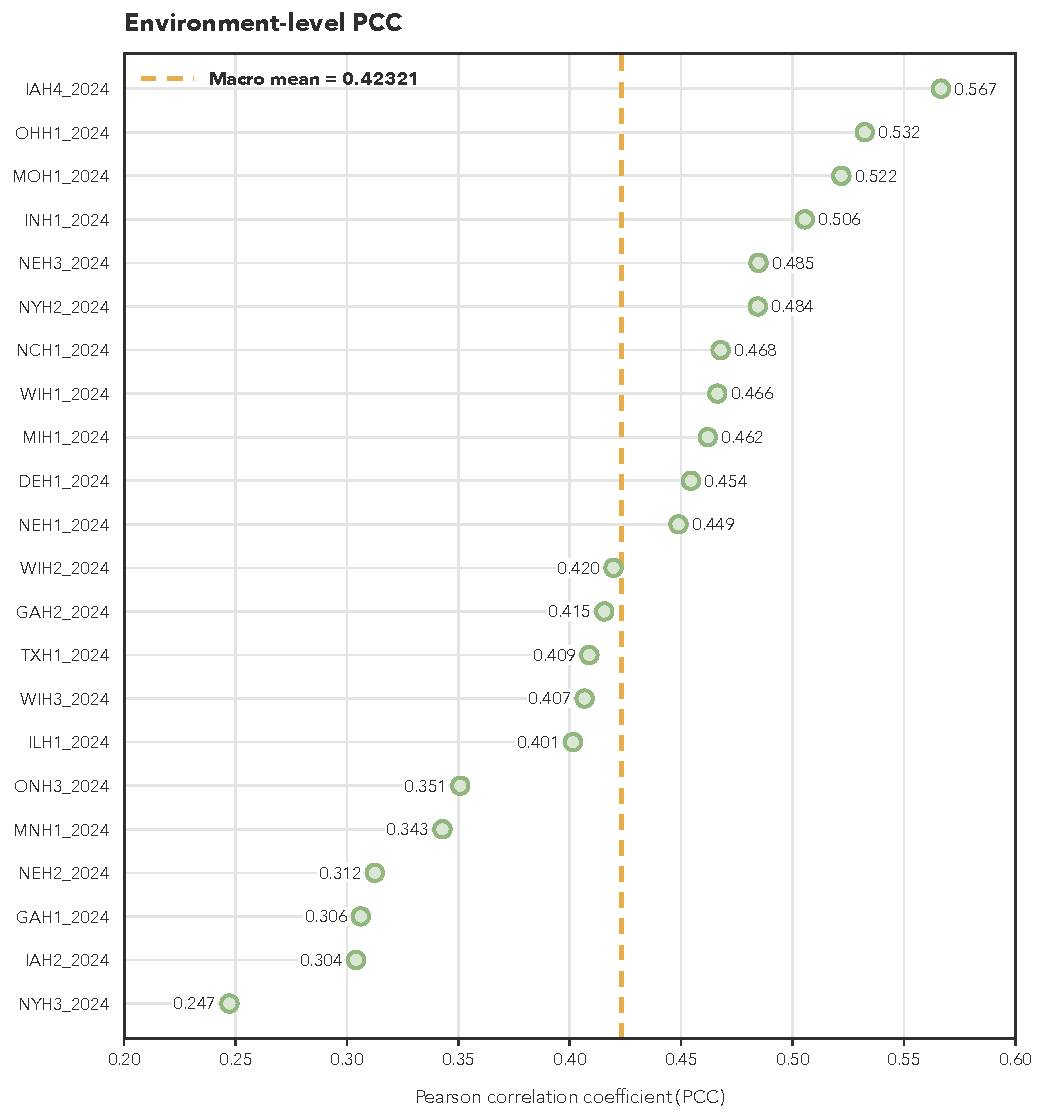
\includegraphics[width=\linewidth]{figures/gxe-tf/environment-level-pcc.pdf}
    \caption{Environment-level Pearson correlation coefficients (PCCs) for the selected FullTransformer checkpoint on the 2024 retrospective benchmark. Green points show PCC for each of the 22 environments in the benchmark cohort, ordered from highest to lowest. The dashed orange line marks the macro environment PCC of 0.423. Point labels show values rounded to three decimals.}
    \label{fig:ch3-environment-pcc}
\end{figure}

We also examined the upper and lower ends of the environment-level PCC distribution. The environment with the highest PCC was \texttt{IAH4\_2024}, with a PCC of $0.567$. The second-highest PCC occurred in \texttt{OHH1\_2024}, with a PCC of $0.532$, and the third-highest occurred in \texttt{MOH1\_2024}, with a PCC of $0.522$. In contrast, the environment with the lowest PCC was \texttt{NYH3\_2024}, with a PCC of $0.247$. The second-lowest was \texttt{IAH2\_2024}, with a PCC of $0.304$, and the third-lowest was \texttt{GAH1\_2024}, with a PCC of $0.306$. The difference between the highest and lowest environment-level PCC values was $0.319$, demonstrating considerable heterogeneity in model performance across environments.

\subsection{Competition Context} \comment{gotta make sure this is up-to-date with the new manuscript draft}
To contextualize the reported FullTransformer result, we compared it with the leading competing entries on the 2024 G2F G$\times$E Prediction Competition EvalAI leaderboard \cite{g2f-2024-evalai-leaderboard}. The competition ranked submissions using the macro environment PCC, the same primary metric used in our retrospective benchmark \cite{g2f-2024-competition}. Several leaderboard entries marked as \enquote{not competing} were omitted from this comparison \comment{update this: several entries were marked as not competing, and several were disqualified}. The FullTransformer achieved a PCC of $0.423$, which would have ranked third among the competing entries shown in Table~\ref{tab:ch3-external-results}. This score was $0.003$ lower than the fifth-place score and $0.027$ lower than the winning score. \comment{fix these numbers} Because the FullTransformer was evaluated after the competition and was not submitted, this placement is a retrospective comparison rather than an official result. Its proximity to the second-place score nevertheless indicates that the architecture was competitive with the leading competition entries.

\begin{table}[htbp]
    \centering
    \footnotesize
    \begin{tabularx}{\textwidth}{@{}c X c@{}}
        \toprule
        Rank & Entry & Competition PCC \\
        \midrule
        1 & Naaa & 0.45005 \\
        2 & NJUST\_KMG1 & 0.44402 \\
        3 & PARaBra & 0.43710 \\
        4 & transform(Base) & 0.42605 \\
        5 & The Cornquerors & 0.42574 \\
        (6) & FullTransformer (retrospective) & 0.42321 \\
        \bottomrule
    \end{tabularx}
    \caption{\comment{change the table to remove DQ'ed scores} Comparison of the FullTransformer result with the five leading competing entries on the 2024 G$\times$E Prediction Competition EvalAI leaderboard. Entries explicitly marked as not competing were omitted. The FullTransformer score is a retrospective comparison and was not an official competition submission; its rank is given in parentheses to mark the position the score would have taken.}
    \label{tab:ch3-external-results}
\end{table}


\section{Discussion}
This study tested whether a unified representation of marker and environmental tokens could support maize G$\times$E yield prediction more effectively than branch-based late fusion. Our results support early cross-modal interaction as a useful design choice and show that prediction rank and absolute scale require distinct treatment. The final FullTransformer combined these choices and achieved a competitive retrospective macro environment PCC of $0.423$ on the 2024 competition benchmark.

Unlike a late-fusion architecture, the FullTransformer places marker and environmental tokens in one sequence before either modality enters a separate encoder. This design gives each marker token a direct attention connection to every environmental token; thus, the model can form cross-modal representations before separate encoders can discard information needed for later interactions. Prior multimodal G$\times$E methods often use separate encoders and late fusion \cite{montesinos2024multimodal,shook2021crop}, so the comparison addresses a common design choice. The higher PCC and lower MSE of the unified control were consistent with this rationale. The unified model also reached the higher score with about half the trainable parameters of the branch-based late-fusion model, so capacity does not explain the difference. However, one seed and several component differences prevent a causal attribution to early fusion alone.

Objective choice exposed a practical trade-off between within-environment selection and absolute yield prediction. Macro environment PCC emphasizes whether the model preserves relative yield variation within each environment. By contrast, macro environment MSE penalizes errors in yield units, including errors in scale and offset. These metrics therefore support different uses: PCC supports hybrid selection within a trial, whereas MSE supports yield estimates on an absolute scale. The environment-conditioned affine head recovered part of the scale gap through a positive scale and shift that preserved within-environment PCC. In the near-matched comparison, this calibration reduced macro environment MSE by $45.2\%$, which supports separate correlation and scale targets. However, the calibrated model's macro environment MSE was still 3.8$\times$ higher than that of the global MSE-trained model. That model in turn reached a macro environment PCC of only $0.305$, $0.118$ below the calibrated model, so it would rank hybrids poorly within a trial. Calibration therefore narrowed the trade-off rather than removing it.

The mean benchmark PCC concealed substantial variation among the eligible 2024 environments. Although every environment had positive PCC, the model did not provide uniform reliability across environments. This variation could reflect differences in environmental complexity, data quality, sample composition, or other unmeasured factors, but this study did not test these explanations. These results show that model assessment requires both aggregate and environment-level metrics.

The retrospective placement below the two leading entries supports competitiveness, but it does not constitute an official competition result. Public leaderboard records do not describe each submission method, so score differences cannot identify which architecture choices caused the placement. The 2022 G2F competition also found no clear advantage for one model family \cite{g2f-maize-2025}. This broader pattern suggests that the FullTransformer score establishes method viability, not architecture superiority. \comment{can we use what we know in the unifinished manuscript?}

\subsection{Limitations and Future Work}
Each highlighted comparison used one seed, so the study could not estimate variation across random initialization. Future work should evaluate multiple seeds to quantify variation across model initializations.

The architecture comparison matched principal training settings, but its two designs differed in several components. The calibration comparison also used near-matched runs from adjacent commits. These comparisons therefore provide descriptive evidence rather than isolated causal effects. Future work should use controlled single-component ablations across multiple seeds.

The study used the 2024 labels for several model comparisons, so the benchmark was not an untouched external test set. The reported scores therefore describe retrospective benchmark performance, not a prospective competition submission. After method development, we will evaluate the FullTransformer on a future G2F season or another untouched benchmark.

Leave-environment-out validation holds out whole environments from the pre-2024 years, so it measures spatial interpolation for hybrids that the model has already seen. The 2024 benchmark posed a different problem. All 22 of its environments were new to the model, and $87.6\%$ of its hybrids were crosses absent from the training data. We therefore selected the reported checkpoint with a criterion that does not completely track benchmark performance. An improvement measured under leave-environment-out validation need not transfer to novel crosses in a novel year. Future work should build a validation design that reproduces the novel-cross and novel-year structure of the benchmark.

The tester composition of the benchmark was also highly asymmetric. PHP02 accounted for 5,119 of the 9,486 rows and LH287 for 3,716, which left 651 rows for all other testers. The reported scores therefore describe performance on crosses to two tester backgrounds. They provide little evidence about hybrids with other testers.

Access to compute constrained the design of the study. Training the reported model required 32 GPUs across four nodes of a shared supercomputer, and every run depended on an allocation award and on queue scheduling. This constraint, rather than the cost of any single run, is the practical reason the highlighted comparisons use single runs rather than replicated seeds. The reported result also rests on one checkpoint and its captured run configuration. We will archive that checkpoint, its configuration, the benchmark predictions, and the metric output with the manuscript.

In addition to the future work that is necessary to address the study's limitations, we outline several directions for further model improvement. First, we plan to evaluate the new reproducible data pipeline and feature tokenization options. The pipeline creates traceable and repeatable data from the raw competition files, including fixed imputation, filters, feature order, and data splits. This structure will also support controlled tests of alternative preprocessing choices. The tokenization options will support feature-aware representations for temperature, precipitation, soil, management, and other environmental covariates.

Furthermore, we plan to add temporal detail to the weather representation. The current model uses seasonal weather summaries, which can hide the date and crop stage of a weather event. Instead, we plan to test a weather encoder that can process daily weather sequences from planting to harvest. This approach will align weather features by days after planting rather than calendar dates. Development measures, such as growing degree days, could provide a closer link to crop stage. A transformer, RNN, or LSTM will convert the daily sequence into one or more weather tokens.

The model can then use attention to combine these tokens with soil, management, and marker tokens. We will compare seasonal weather summaries, temporal weather tokens, and their combination for G$\times$E prediction.

In addition to improving data and environmental representations, we plan to test whether external parental representations improve predictions for unseen hybrids. Currently, the model uses a shared learned dosage embedding across markers, with positional codes that identify loci. We plan to evaluate external parental information, such as parent genotypes, pedigree or relationship data, and known tester identity. Parent genotype data may overlap with hybrid marker data, but direct parental representations could expose inheritance and relationships more clearly.

We will compare hybrid markers alone with parent identity tokens, parent genotype representations, pedigree data, and combining-ability features. We will calculate any combining-ability features from the fit partition only to prevent target leakage. We will report performance on novel crosses, known crosses, and major testers.

Two further directions follow from the results reported above. The affine calibration head was trained as a low-weight auxiliary objective, so we will test whether a stronger calibration objective reduces macro environment MSE further without harming macro environment PCC. We will also test whether environmental complexity, data quality, or sample composition explain the variation in environment-level PCC, and whether environment-specific adaptation or calibrated uncertainty estimates improve reliability across environments.

All future comparisons will use multiple paired seeds and report mean scores, standard deviations, and paired differences to measure effects beyond seed variation.
